%! TeX Program = lualatex
\documentclass[english,aspectratio=169,t]{beamer}
\usepackage{babel}
\usepackage{graphicx}
\usepackage{amsmath,amssymb}
\usepackage{booktabs}
\usepackage{listings}
\usepackage{fancyvrb}
\usepackage{xcolor}
\usepackage{tikz}
\usetikzlibrary{arrows.meta,positioning,shapes.geometric,fit,calc}
\usetheme{Comsys}

\graphicspath{{assets/}{assets/ui/}{assets/veritesting/}{assets/experiments/}}
\definecolor{codekw}{RGB}{0,78,140}
\definecolor{codecomment}{RGB}{92,99,112}
\definecolor{codestring}{RGB}{34,120,76}
\definecolor{codeconst}{RGB}{152,72,7}
\lstdefinestyle{code}{
  basicstyle=\ttfamily\scriptsize,
  columns=fullflexible,
  keepspaces=true,
  showstringspaces=false,
  frame=single,
  breaklines=true,
  tabsize=2,
  keywordstyle=\color{codekw}\bfseries,
  commentstyle=\color{codecomment}\itshape,
  stringstyle=\color{codestring},
  numberstyle=\tiny\color{codecomment}
}
\lstdefinestyle{cppcode}{
  style=code,
  language=C++,
  keywordstyle=\color{codekw}\bfseries,
  commentstyle=\color{codecomment}\itshape,
  stringstyle=\color{codestring}
}
\lstdefinestyle{mircode}{
  style=code,
  language=MIR,
  keywordstyle=\color{codekw}\bfseries,
  moredelim=[is][\color{codeconst}]{\#}{\ },
}
\lstdefinestyle{terminal}{
  style=code,
  basicstyle=\ttfamily\fontsize{4.4}{4.8}\selectfont,
  keywordstyle=\color{black},
  commentstyle=\color{black},
  stringstyle=\color{black}
}
\lstdefinestyle{tinycode}{style=code,basicstyle=\ttfamily\tiny}
\lstdefinelanguage{MIR}{
  morekeywords={param,goto,return,ifTrue,ifFalse,Lloop,Lskip,Lnext,Lend,Ljoin,Lneg,Lhot},
  sensitive=true,
  morecomment=[l]{//}
}
\lstset{style=code}
\newcommand{\sourcefoot}[1]{\vfill\tiny\color{gray}#1}
\newcommand{\maybegraphic}[2][]{\IfFileExists{#2}{\includegraphics[#1]{#2}}{\fbox{\parbox[c][.44\textheight][c]{.9\linewidth}{\centering Missing asset:\\texttt{\detokenize{#2}}}}}}
\newcommand{\statebox}[3]{\begin{tabular}{@{}ll@{}}$\ell$ & #1 \\ $\pi$ & #2 \\ $\mu$ & #3\end{tabular}}
\newcommand{\paper}[1]{\textbf{#1}}
\newenvironment{truebranchblock}[1]{%
  \begingroup
  \setbeamercolor{block title}{fg=white,bg=green!45!black}%
  \setbeamercolor{block body}{fg=black,bg=green!9}%
  \begin{block}{#1}%
}{\end{block}\endgroup}
\newenvironment{falsebranchblock}[1]{%
  \begingroup
  \setbeamercolor{block title}{fg=white,bg=red!60!black}%
  \setbeamercolor{block body}{fg=black,bg=red!7}%
  \begin{block}{#1}%
}{\end{block}\endgroup}
\newenvironment{sourcespaperblock}[1]{%
  \begingroup
  \setbeamercolor{block title}{fg=white,bg=blue!65!black}%
  \setbeamercolor{block body}{fg=black,bg=blue!6}%
  \begin{block}{#1}%
}{\end{block}\endgroup}
\newenvironment{sourcesprojectblock}[1]{%
  \begingroup
  \setbeamercolor{block title}{fg=white,bg=green!45!black}%
  \setbeamercolor{block body}{fg=black,bg=green!8}%
  \begin{block}{#1}%
}{\end{block}\endgroup}
\tikzset{
  box/.style={draw, rounded corners, align=center, minimum height=0.78cm, inner sep=5pt},
  branch/.style={diamond, draw, aspect=2.0, align=center, inner sep=1.5pt},
  line/.style={-{Latex[length=2.0mm]}, thick},
  smallbox/.style={draw, rounded corners, align=center, inner sep=3.5pt, font=\small},
  qbox/.style={draw, rounded corners, align=center, inner sep=7pt, fill=blue!7, minimum width=3.2cm}
}

\title[State Merging]{State Merging in Symbolic Execution}
\author{Yaroslav Riabtsev}
\authorextra{Communication and Distributed Systems}
\subtitle{MIR dumps, query relevance, and compact summaries}
\date{July 2026}

\begin{document}
\titleframe

\begin{frame}[fragile]{KLEE run vs. internal analysis}
  \begin{columns}[T,onlytextwidth]
    \column{.56\textwidth}
      \textbf{KLEE input program}\par\vspace{-0.3em}
      \lstinputlisting[style=cppcode,basicstyle=\ttfamily\fontsize{4.8}{5.2}\selectfont,firstline=1,lastline=18]{assets/klee/shown.cpp}
      \vspace{0.2em}
      \textbf{Raw KLEE output excerpt}\par\vspace{-0.3em}
      \lstinputlisting[style=terminal]{assets/klee/terminalexcerpt.txt}
    \column{.42\textwidth}
      \textbf{Internal analysis view}\par\vspace{0.2em}
      \centering
      \maybegraphic[width=\linewidth,height=.61\textheight,keepaspectratio]{assets/ui/test13_overview.png}
      \par\vspace{0.35em}
      {\scriptsize\href{https://yaryabtsev.github.io/compilers-course/}{\texttt{yaryabtsev.github.io/compilers-course/}}}
  \end{columns}
\end{frame}

\begin{frame}[fragile]{Repeated symbolic branching}
  \begin{columns}[T,onlytextwidth]
    \column{.48\textwidth}
      \textbf{C++ source}\par\vspace{-0.35em}
      \lstinputlisting[style=cppcode,basicstyle=\ttfamily\fontsize{5.1}{5.6}\selectfont]{assets/data/snippets/countmatches.cpp}
      \vspace{0.15em}
      \textbf{MIR dump}\par\vspace{-0.35em}
      \lstinputlisting[style=mircode,basicstyle=\ttfamily\fontsize{5.1}{5.6}\selectfont]{assets/data/snippets/test17loop.mir}
    \column{.49\textwidth}
      \textbf{Path histories}\par\vspace{0.35em}
      \centering
      \resizebox{.94\linewidth}{!}{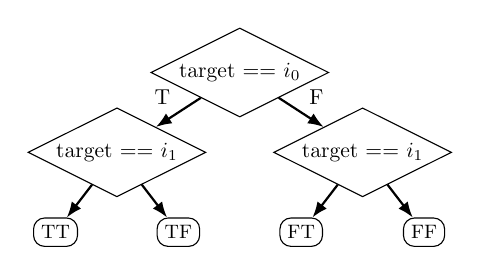
\begin{tikzpicture}[scale=.78,transform shape]
        \node[branch] (root) at (0,0) {target == $i_0$};
        \node[branch] (left) at (-2.0,-1.3) {target == $i_1$};
        \node[branch] (right) at (2.0,-1.3) {target == $i_1$};
        \node[smallbox] (tt) at (-3.0,-2.6) {TT};
        \node[smallbox] (tf) at (-1.0,-2.6) {TF};
        \node[smallbox] (ft) at (1.0,-2.6) {FT};
        \node[smallbox] (ff) at (3.0,-2.6) {FF};
        \draw[line] (root) -- node[above left]{T} (left);
        \draw[line] (root) -- node[above right]{F} (right);
        \draw[line] (left) -- (tt);
        \draw[line] (left) -- (tf);
        \draw[line] (right) -- (ft);
        \draw[line] (right) -- (ff);
      \end{tikzpicture}}
      \vspace{0.65em}
      \Large\[1,2,4,8,\ldots,2^k\]
  \end{columns}
\end{frame}

\begin{frame}[fragile]{One branch and one join}
  \begin{columns}[T,onlytextwidth]
    \column{.48\textwidth}
      \textbf{C++ fragment}\par\vspace{-0.35em}
      \lstinputlisting[style=cppcode,basicstyle=\ttfamily\fontsize{6.1}{6.7}\selectfont]{assets/data/snippets/itehotbranch.cpp}
      \vspace{0.25em}
      \textbf{MIR dump}\par\vspace{-0.35em}
      \lstinputlisting[style=mircode,basicstyle=\ttfamily\fontsize{5.7}{6.2}\selectfont]{assets/data/snippets/test13branch.mir}
    \column{.49\textwidth}
      \textbf{CFG}\par\vspace{0.55em}
      \centering
      \resizebox{.88\linewidth}{!}{%
      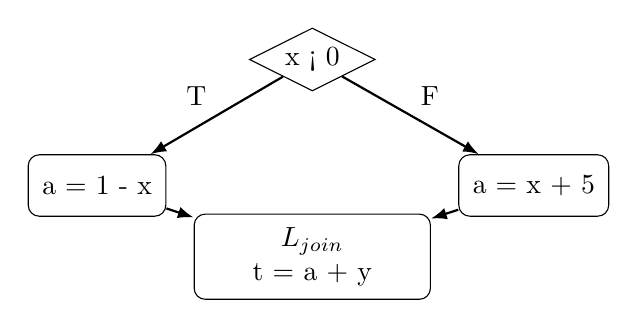
\begin{tikzpicture}[node distance=1.0cm and 1.45cm]
        \node[branch] (split) {x < 0};
        \node[box, below left=of split] (neg) {a = 1 - x};
        \node[box, below right=of split] (pos) {a = x + 5};
        \node[box, below=1.55cm of split, minimum width=3.0cm] (join) {$L_{join}$\\t = a + y};
        \draw[line] (split) -- node[above left]{T} (neg);
        \draw[line] (split) -- node[above right]{F} (pos);
        \draw[line] (neg) -- (join);
        \draw[line] (pos) -- (join);
      \end{tikzpicture}}
  \end{columns}
\end{frame}

\begin{frame}{Two states in the worklist}
  \centering
  \[s=(\ell,\pi,\mu)\]
  \begin{columns}[T,onlytextwidth]
    \column{.47\textwidth}
      \begin{truebranchblock}{True branch: $s_1$}
        \statebox{$L_{join}$}{$x<0$}{$a\mapsto 1-x$}
      \end{truebranchblock}
    \column{.47\textwidth}
      \begin{falsebranchblock}{False branch: $s_2$}
        \statebox{$L_{join}$}{$\neg(x<0)$}{$a\mapsto x+5$}
      \end{falsebranchblock}
  \end{columns}
  \vspace{0.35em}
  \begin{block}{Worklist $W$}
    \centering
    \Large
    $\text{front}\;\longrightarrow\;\boxed{s_1}\;\boxed{s_2}\;\boxed{\cdots}$
    \hfill
    \normalsize $(\ell,\pi,\mu)=pickNext(W)$
  \end{block}
\end{frame}

\begin{frame}{Merging the same two states}
  \begin{columns}[T,onlytextwidth]
    \column{.47\textwidth}
      \begin{truebranchblock}{True branch: $s_1$}
        \statebox{$L_{join}$}{$\pi_1=x<0$}{$a\mapsto 1-x$}
      \end{truebranchblock}
    \column{.47\textwidth}
      \begin{falsebranchblock}{False branch: $s_2$}
        \statebox{$L_{join}$}{$\pi_2=\neg(x<0)$}{$a\mapsto x+5$}
      \end{falsebranchblock}
  \end{columns}
  \vspace{-0.1em}
  \begin{center}
    \Large $\Downarrow$\quad
    \normalsize merge-compatible: same location $L_{join}$
  \end{center}
  \vspace{-0.3em}
  \begin{block}{Merged state}
    \begin{columns}[T,onlytextwidth]
      \column{.47\textwidth}
        \statebox{$L_{join}$}{$\pi_1\lor\pi_2$}{$a\mapsto \operatorname{ite}(\pi_1,1-x,x+5)$}
      \column{.49\textwidth}
        \[\pi=\pi_1\lor\pi_2\]
        \vspace{-0.8em}
        \[\mu(a)=\operatorname{ite}(\pi_1,1-x,x+5)\]
    \end{columns}
  \end{block}
\end{frame}

\begin{frame}[fragile]{Sharing symbolic expressions}
  \begin{columns}[T,onlytextwidth]
    \column{.73\textwidth}
      \centering
      \includegraphics[width=\linewidth,height=.56\textheight,keepaspectratio]{assets/veritesting/veritesting_figure4_hash_consing.pdf}
    \column{.24\textwidth}
      \textbf{Straight-line input}\par\vspace{0.35em}
      \begin{lstlisting}[style=cppcode,basicstyle=\ttfamily\fontsize{6.0}{6.8}\selectfont]
x = s; // s is symbolic
x = x + x;
x = x + x;
x = x + x;
assert(x == 42);
      \end{lstlisting}
  \end{columns}
  \vspace{0.3em}
  \centering
  \small\emph{Figure 4: Hash consing example. Top-left: naively generated formula. Top-right: hash-consed formula.}
  \sourcefoot{Avgerinos et al., Enhancing Symbolic Execution with Veritesting, ICSE 2014, Fig. 4.}
\end{frame}



\begin{frame}[fragile]{Formula growth after the merge}
  \begin{columns}[T,onlytextwidth]
    \column{.31\textwidth}
      \textbf{Remaining code}\par\vspace{-0.3em}
      \begin{lstlisting}[style=cppcode,basicstyle=\ttfamily\fontsize{5.15}{5.75}\selectfont]
int a;
if (x < 0) {
  a = 1 - x;
} else {
  a = x + 5;
}

int t = a + y;
int r;
if (t > 0)
  r = t + 1;
else
  r = y + 1;

      \end{lstlisting}
    \column{.67\textwidth}
      \small
      \textbf{Merged value}
      \[
        a=\operatorname{ite}(x<0,\;1-x,\;x+5)
      \]
      \vspace{-0.75em}
      \textbf{Substitute directly into $t$}
      \[
        t=\operatorname{ite}(x<0,\;1-x,\;x+5)+y
      \]
      \vspace{-0.75em}
      \textbf{Substitute directly into $r$}
      {\scriptsize
      \[
      \begin{aligned}
      r=\operatorname{ite}(&\operatorname{ite}(x<0,1-x,x+5)+y>0,\\
                           &\operatorname{ite}(x<0,1-x,x+5)+y+1,\\
                           &y+1)
      \end{aligned}
      \]
      }
      \vspace{-0.85em}
      \textbf{Push additions into the $ite$ branches}
      {\scriptsize
      \[
      \begin{aligned}
      r=\operatorname{ite}(&\operatorname{ite}(x<0,1-x+y,x+5+y)>0,\\
                           &\operatorname{ite}(x<0,2-x+y,x+6+y),\\
                           &y+1)
      \end{aligned}
      \]
      }
  \end{columns}
  \vspace{-0.45em}
  \begin{center}\small fewer states, repeated symbolic subexpressions\end{center}
\end{frame}


\begin{frame}[fragile]{Before QCE: the merge question}
  \begin{columns}[T,onlytextwidth]
    \column{.31\textwidth}
      \textbf{Remaining code}\par\vspace{-0.3em}
      \begin{lstlisting}[style=cppcode,basicstyle=\ttfamily\fontsize{5.15}{5.75}\selectfont]
int a;
if (x < 0) {
  a = 1 - x;
} else {
  a = x + 5;
}
// Ljoin: candidate merge of a
int t = a + y;
int r;
if (t > 0)
  r = t + 1;
else
  r = y + 1;
// Lend: candidate merge of r
      \end{lstlisting}
      \vspace{0.25em}
      {\scriptsize
      \[
      a\text{ differs at }L_{join}
      \Rightarrow
      t=a+y
      \Rightarrow
      t>0
      \]
      }
    \column{.67\textwidth}
      \centering
      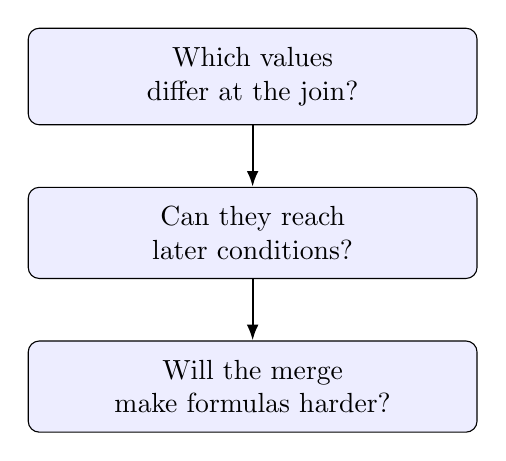
\begin{tikzpicture}[node distance=.78cm]
        \node[qbox, minimum width=5.7cm] (diff) {Which values\\differ at the join?};
        \node[qbox, minimum width=5.7cm, below=of diff] (flow) {Can they reach\\later conditions?};
        \node[qbox, minimum width=5.7cm, below=of flow] (cost) {Will the merge\\make formulas harder?};
        \draw[line] (diff) -- (flow);
        \draw[line] (flow) -- (cost);
      \end{tikzpicture}
  \end{columns}
\end{frame}




\newcommand{\futuredependencydiagram}{%
  \resizebox{0.92\linewidth}{!}{%
  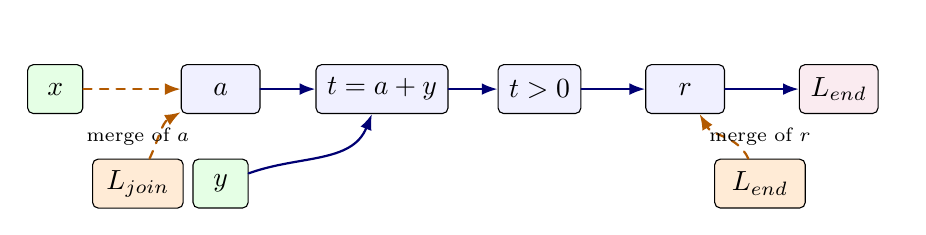
\begin{tikzpicture}[
    dep/.style={draw, rounded corners=2pt, align=center, inner sep=4pt, fill=white, minimum height=.62cm},
    source/.style={dep, fill=green!10, minimum width=.70cm},
    expr/.style={dep, fill=blue!6, minimum width=1.00cm},
    merge/.style={dep, fill=orange!16, minimum width=1.15cm},
    final/.style={dep, fill=purple!8, minimum width=1.00cm},
    note/.style={font=\scriptsize, align=center},
    flow/.style={-{Latex[length=2.0mm]}, thick, blue!45!black},
    diff/.style={-{Latex[length=2.0mm]}, thick, orange!70!black, dashed},
    every path/.style={line cap=round}
  ]
    \path[use as bounding box] (-0.35,-1.08) rectangle (10.70,1.20);
    \node[source] (x) at (0,0.42) {$x$};
    \node[expr] (a) at (2.10,0.42) {$a$};
    \node[source] (y) at (2.10,-0.78) {$y$};
    \node[expr] (t) at (4.15,0.42) {$t=a+y$};
    \node[expr] (cond) at (6.15,0.42) {$t>0$};
    \node[expr] (r) at (8.00,0.42) {$r$};
    \node[final] (end) at (9.95,0.42) {$L_{end}$};
    \node[merge] (m1) at (1.05,-0.78) {$L_{join}$};
    \node[merge] (m2) at (8.95,-0.78) {$L_{end}$};

    \draw[diff] (x) -- (a);
    \draw[flow] (a) -- (t);
    \draw[flow] (y) to[out=20,in=-112] (t);
    \draw[flow] (t) -- (cond);
    \draw[flow] (cond) -- (r);
    \draw[flow] (r) -- (end);
    \draw[diff] (m1) to[out=65,in=-150] (a);
    \draw[diff] (m2) to[out=115,in=-60] (r);

    \node[note, above=.05cm of m1] {merge of $a$};
    \node[note, above=.05cm of m2] {merge of $r$};
  \end{tikzpicture}}
}
\newcommand{\futuredependencysection}{%
  \textbf{Future dependency}\par\vspace{0.08em}%
  \centering
  \futuredependencydiagram
}






\begin{frame}[fragile]{Candidate merge points}
  \begin{minipage}[t][0.38\textheight][t]{\textwidth}
  \begin{columns}[T,onlytextwidth]
    \column{.48\textwidth}
      \textbf{Candidate at $L_{join}$}\par\vspace{-0.3em}
      \begin{lstlisting}[style=cppcode,basicstyle=\ttfamily\fontsize{5.3}{5.85}\selectfont]
int a;
if (x < 0) {
  a = 1 - x;
} else {
  a = x + 5;
}
// Ljoin: candidate merge of a
      \end{lstlisting}
    \column{.48\textwidth}
      \textbf{Candidate at $L_{end}$}\par\vspace{-0.3em}
      \begin{lstlisting}[style=cppcode,basicstyle=\ttfamily\fontsize{5.3}{5.85}\selectfont]
int t = a + y;
int r;
if (t > 0) {
  r = t + 1;
} else {
  r = y + 1;
}
// Lend: candidate merge of r
      \end{lstlisting}
  \end{columns}
  \end{minipage}
  \vspace{0.10em}
  \futuredependencysection
\end{frame}






\begin{frame}{What changes at each candidate?}
  \begin{minipage}[t][0.38\textheight][t]{\textwidth}
  \begin{columns}[T,onlytextwidth]
    \column{.48\textwidth}
      \begin{block}{At $L_{join}$}
        \begin{tabular}{@{}ll@{}}
          differing source of $a$ & $\{x\}$\\
          future condition depends on & $\{x,y\}$\\
          overlap & $\{x\}$
        \end{tabular}
      \end{block}
    \column{.48\textwidth}
      \begin{block}{At $L_{end}$}
        \begin{tabular}{@{}ll@{}}
          $r$ differs & yes\\
          future condition & none\\
          overlap & $\varnothing$
        \end{tabular}
      \end{block}
  \end{columns}
  \end{minipage}
  \vspace{0.10em}
  \futuredependencysection
\end{frame}







\begin{frame}{Project dump view}
  \scriptsize
  \textbf{Merge-risk table}\par\vspace{0.16em}
  \begin{center}
  \resizebox{0.82\textwidth}{!}{%
  \begin{tabular}{|l|l|l|l|l|l|}
    \hline
    Join & Value & Diff sources & Future hot & Overlap & Result\\
    \hline
    $L_{join}$ & $a$ & $\{x\}$ & $\{x,y\}$ & $\{x\}$ & mixed\\
    \hline
    $L_{end}$ & $r$ & $\{x,y\}$ & $\varnothing$ & $\varnothing$ & no future query\\
    \hline
  \end{tabular}}
  \end{center}

  \vspace{0.22em}
  \textbf{Dependency recovery vs. manual QCE oracle}\par\vspace{0.16em}
  \begin{center}
  \resizebox{\textwidth}{!}{%
  \begin{tabular}{|l|l|l|l|}
    \hline
    Analysis & Recovered for $t>0$ & What is added & Oracle L1\\
    \hline
    Manual QCE oracle & $\{x,y\}$ & original C-relation + q-recurrence & reference\\
    \hline
    Syntactic & $\{t\}$ & direct branch operands & 10\\
    \hline
    Local & $\{a,y\}$ & same-block def-use expansion & 5\\
    \hline
    CFG & $\{x,y\}$ & propagation through predecessors and joins & 0\\
    \hline
    Versioned & $\{x_0,y_0\}$ & definition-sensitive source tracking & 0\\
    \hline
  \end{tabular}}
  \end{center}

  \vspace{0.12em}
  {\tiny Oracle L1 is computed in the source-variable domain; $x_0,y_0$ are normalized to $x,y$.}
\end{frame}



\begin{frame}{QCE shape from the paper}
  \begin{columns}[T,onlytextwidth]
    \column{.58\textwidth}
      {\scriptsize
      \[
      q(\ell,c)=
      \begin{cases}
      \beta q(succ(\ell),c)+\beta q(\ell',c)+c(\ell,e), & instr(\ell)=if(e)\ goto\ \ell'\\
      0, & instr(\ell)=halt\\
      q(succ(\ell),c), & \text{otherwise}
      \end{cases}
      \]
      }
      \[
      Q_t(\ell)=q(\ell,c_t),\qquad
      Q_{add}(\ell,v)=q(\ell,c_{add,v})
      \]
      \[
      Hot(\ell)=\{v\mid Q_{add}(\ell,v)>\alpha Q_t(\ell)\}
      \]
    \column{.39\textwidth}
      {\small
      \begin{block}{Parameters}
        \begin{tabular}{@{}ll@{}}
          $\alpha>0$ & threshold\\
          $\beta\in(0.5,1)$ & attenuation\\
          $\kappa\in\mathbb{N}$ & preview bound
        \end{tabular}
      \end{block}
      }
      \vspace{0.25em}
      {\scriptsize dump run: $\alpha=0.35$, $\beta=0.50$ boundary value\par}
      \vspace{0.35em}
      {\small The formulas on the left are the paper-shaped reference. }
  \end{columns}
  \sourcefoot{Kuznetsov et al., Efficient State Merging in Symbolic Execution, PLDI 2012.}
\end{frame}

\begin{frame}{Veritesting regions and transition points}
  \begin{columns}[T,onlytextwidth]
    \column{.33\textwidth}
      \small
      \paper{Efficient merging}\\
      state-level merge and QCE\\[0.9em]
      \paper{Veritesting}\\
      calls and returns often become transition points\\[0.9em]
      \paper{Java Ranger}\\
      dynamically inline method regions
    \column{.65\textwidth}
      \centering
      \includegraphics[width=\linewidth,height=.54\textheight,keepaspectratio]{assets/veritesting/veritesting_figure1_transition_points.pdf}
      \vspace{0.2em}

      {\scriptsize\emph{Veritesting on a program fragment with loops and system calls. (a) Recovered CFG. (b) CFG after transition point identification \& loop unrolling. Unreachable nodes are shaded.}}
  \end{columns}
  \sourcefoot{Avgerinos et al., Enhancing Symbolic Execution with Veritesting, ICSE 2014, Fig. 1.}
\end{frame}

\begin{frame}[fragile]{Java call chain: raw bytecode view}
  \begin{columns}[T,onlytextwidth]
    \column{.33\textwidth}
      \small
      \paper{Efficient merging}\\
      state-level merge and QCE\\[0.9em]
      \paper{Veritesting}\\
      calls and returns often become transition points\\[0.9em]
      \paper{Java Ranger}\\
      dynamically inline method regions
    \column{.65\textwidth}
      \VerbatimInput[fontsize=\fontsize{4.6}{4.9}\selectfont,frame=single]{assets/java/javachain.txt}
  \end{columns}
  \sourcefoot{Right side: raw javap excerpt generated locally. Java Ranger motivates dynamic method-region inlining for small dynamically dispatched Java methods.}
\end{frame}
\begin{frame}{Loops across the papers}
  \centering
  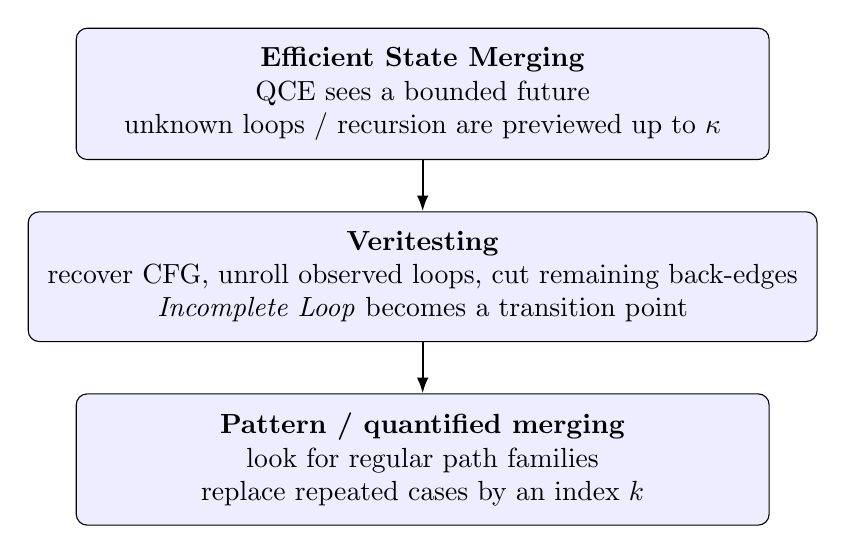
\begin{tikzpicture}[node distance=.65cm]
    \node[qbox, minimum width=8.8cm] (esm) {\textbf{Efficient State Merging}\\QCE sees a bounded future\\unknown loops / recursion are previewed up to $\kappa$};
    \node[qbox, minimum width=8.8cm, below=of esm] (veri) {\textbf{Veritesting}\\recover CFG, unroll observed loops, cut remaining back-edges\\\emph{Incomplete Loop} becomes a transition point};
    \node[qbox, minimum width=8.8cm, below=of veri] (quant) {\textbf{Pattern / quantified merging}\\look for regular path families\\replace repeated cases by an index $k$};
    \draw[line] (esm) -- (veri);
    \draw[line] (veri) -- (quant);
  \end{tikzpicture}
\end{frame}




\begin{frame}[fragile]{Why the two patches matter}
  \begin{columns}[T,onlytextwidth]
    \column{.52\textwidth}
      \textbf{Running example variant}\\[-0.15em]
\begin{lstlisting}[style=cppcode,basicstyle=\ttfamily\fontsize{5.6}{6.1}\selectfont]
int count_matches(int i, int n, int* target) {
  int matches = 0;

  while (i < n) {
    if (target[matches] == i) {
      matches = matches + 1;
    } else {
      matches = matches + 0;
    }

    i = i + 1;
  }

  return matches;
}
\end{lstlisting}
    \column{.45\textwidth}
      \textbf{Two conceptual patches}\par\vspace{0.45em}
      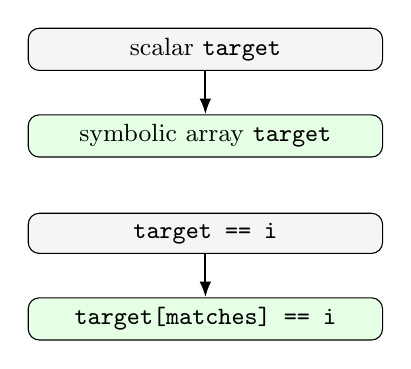
\begin{tikzpicture}[node distance=.55cm]
        \node[smallbox, fill=gray!8, minimum width=4.5cm] (old1) {scalar \texttt{target}};
        \node[smallbox, fill=green!10, below=of old1, minimum width=4.5cm] (new1) {symbolic array \texttt{target}};
        \draw[line] (old1) -- (new1);
        \node[smallbox, fill=gray!8, below=.70cm of new1, minimum width=4.5cm] (old2) {\texttt{target == i}};
        \node[smallbox, fill=green!10, below=of old2, minimum width=4.5cm] (new2) {\texttt{target[matches] == i}};
        \draw[line] (old2) -- (new2);
      \end{tikzpicture}
      \vspace{0.55em}

      \centering
      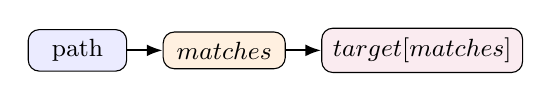
\begin{tikzpicture}[node distance=.30cm]
        \node[smallbox, fill=blue!8, minimum width=1.25cm] (h) {path};
        \node[smallbox, fill=orange!12, right=.45cm of h, minimum width=1.55cm] (m) {$matches$};
        \node[smallbox, fill=purple!8, right=.45cm of m, minimum width=2.55cm] (a) {$target[matches]$};
        \draw[line] (h) -- (m);
        \draw[line] (m) -- (a);
      \end{tikzpicture}
      \vspace{0.45em}

      {\scriptsize bounded $n$, symbolic array contents, sufficient target capacity}
  \end{columns}
\end{frame}



\begin{frame}{Which leaves can be merged together?}
  \centering
  \resizebox{.84\textwidth}{!}{%
  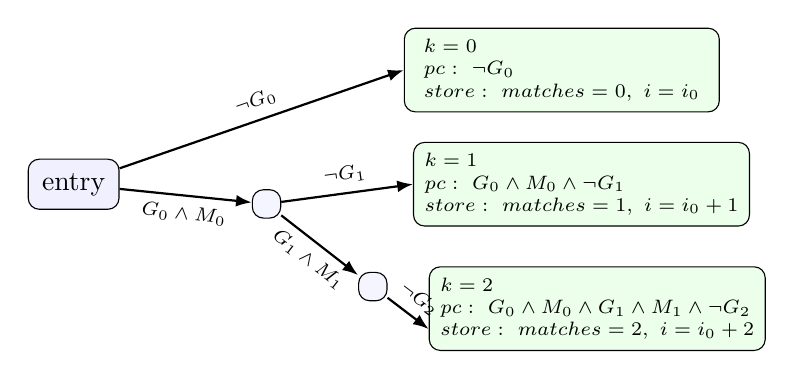
\begin{tikzpicture}[
    root/.style={draw, rounded corners, fill=blue!6, align=center, inner sep=5pt, minimum width=1.15cm},
    leaf/.style={draw, rounded corners, fill=green!8, align=left, inner sep=4pt, font=\scriptsize, minimum width=4.0cm},
    mid/.style={draw, rounded corners, fill=blue!4, inner sep=2.5pt, minimum width=.36cm, minimum height=.36cm},
    edge/.style={-{Latex[length=2mm]}, thick},
    lab/.style={font=\scriptsize, align=center}
  ]
    \node[root] (entry) at (0,0.10) {entry};
    \node[leaf] (k0) at (6.2,1.55) {$k=0$\\$pc:\ \neg G_0$\\$store:\ matches=0,\ i=i_0$};
    \node[mid] (n1) at (2.45,-.15) {};
    \node[leaf] (k1) at (6.45,0.10) {$k=1$\\$pc:\ G_0\land M_0\land\neg G_1$\\$store:\ matches=1,\ i=i_0+1$};
    \node[mid] (n2) at (3.80,-1.20) {};
    \node[leaf] (k2) at (6.65,-1.48) {$k=2$\\$pc:\ G_0\land M_0\land G_1\land M_1\land\neg G_2$\\$store:\ matches=2,\ i=i_0+2$};

    \draw[edge] (entry) -- node[lab, above, sloped] {$\neg G_0$} (k0.west);
    \draw[edge] (entry) -- node[lab, below, sloped] {$G_0\land M_0$} (n1);
    \draw[edge] (n1) -- node[lab, above, sloped] {$\neg G_1$} (k1.west);
    \draw[edge] (n1) -- node[lab, below, sloped] {$G_1\land M_1$} (n2);
    \draw[edge] (n2) -- node[lab, above, sloped] {$\neg G_2$} ($(k2.west)+(0,-0.26)$);
  \end{tikzpicture}}

  \vspace{0.10em}
  {\scriptsize $G_j\equiv i_0+j<n$\quad $M_j\equiv target[j]=i_0+j$\par Selected leaves: same exit, same store domain. Mismatch histories form other groups/fallback.}
\end{frame}


\begin{frame}{How the paper detects a regular partition}
  \begin{columns}[T,onlytextwidth]
    \column{.43\textwidth}
      \textbf{1. Hash conditions by structure}\par\vspace{0.1em}
      \centering
      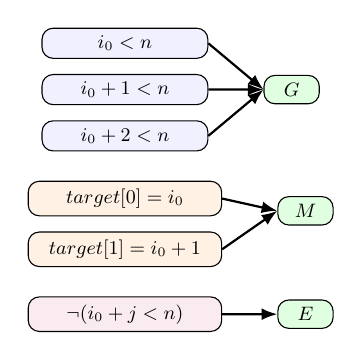
\begin{tikzpicture}[node distance=.25cm, scale=.78, transform shape]
        \node[smallbox, fill=blue!6, minimum width=2.7cm] (g0) {$i_0<n$};
        \node[smallbox, fill=blue!6, below=of g0, minimum width=2.7cm] (g1) {$i_0+1<n$};
        \node[smallbox, fill=blue!6, below=of g1, minimum width=2.7cm] (g2) {$i_0+2<n$};
        \node[smallbox, fill=green!12, right=.9cm of g1, minimum width=.9cm] (G) {$G$};
        \draw[line] (g0.east) -- (G.west);
        \draw[line] (g1.east) -- (G.west);
        \draw[line] (g2.east) -- (G.west);

        \node[smallbox, fill=orange!10, below=.48cm of g2, minimum width=3.15cm] (m0) {$target[0]=i_0$};
        \node[smallbox, fill=orange!10, below=of m0, minimum width=3.15cm] (m1) {$target[1]=i_0+1$};
        \node[smallbox, fill=green!12, right=.9cm of m0, yshift=-.20cm, minimum width=.9cm] (M) {$M$};
        \draw[line] (m0.east) -- (M.west);
        \draw[line] (m1.east) -- (M.west);

        \node[smallbox, fill=purple!8, below=.48cm of m1, minimum width=3.15cm] (e0) {$\neg(i_0+j<n)$};
        \node[smallbox, fill=green!12, right=.9cm of e0, minimum width=.9cm] (E) {$E$};
        \draw[line] (e0.east) -- (E.west);
      \end{tikzpicture}

      \vspace{0.1em}
      {\scriptsize Numeric indices may vary; condition shape and branch polarity are preserved.}
    \column{.55\textwidth}
      \textbf{2. Encode root-to-leaf paths as words}\\[-0.15em]
      \[
      \begin{array}{rcl}
      k=0 &:& W\cdot E\\[0.25em]
      k=1 &:& W\cdot GM\cdot E\\[0.25em]
      k=2 &:& W\cdot GM\cdot GM\cdot E
      \end{array}
      \]
      \vspace{-0.3em}
      \textbf{3. Detect shared regular form}\\[-0.15em]
      \[
        h(\pi(n_k))=\omega_1\omega_2^k\omega_3
      \]
      \begin{center}
      \small
      \begin{tabular}{@{}ll@{}}
        $\omega_1=W$ & common prefix\\
        $\omega_2=GM$ & repeated successful iteration\\
        $\omega_3=E$ & final exit
      \end{tabular}
      \end{center}
  \end{columns}
  \vspace{0.05em}
  \centering
  {\small Regularity is detected in execution-tree constraints, not merely in the CFG loop.}
  \sourcefoot{Trabish et al., \emph{State Merging with Quantifiers in Symbolic Execution}.}
\end{frame}


\begin{frame}{From path pattern to formula pattern}
  \begin{columns}[T,onlytextwidth]
    \column{.38\textwidth}
      \textbf{Observed instances}\\[-0.15em]
      {\scriptsize
      \[
      \begin{array}{rcl}
      k=0 &:& \neg G_0\\[0.25em]
      k=1 &:& G_0\land M_0\land\neg G_1\\[0.25em]
      k=2 &:& G_0\land M_0\land G_1\land M_1\land\neg G_2
      \end{array}
      \]
      }
    \column{.59\textwidth}
      \textbf{Synthesized components}\\[-0.25em]
      {\small
      \[
        \varphi_1=true
      \]
      \[
        \varphi_2(j)=(i_0+j<n)\land(target[j]=i_0+j)
      \]
      \[
        \varphi_3(k)=\neg(i_0+k<n)
      \]
      }
  \end{columns}

  \vspace{-0.2em}
  \textbf{Common schema for each observed $k$}\\[-0.2em]
  {\small
  \[
  tpc(n_k)=\varphi_1\land
  \bigwedge_{j=0}^{k-1}\varphi_2(j)
  \land \varphi_3(k)
  \]
  }

  \vspace{-0.45em}
  \begin{columns}[T,onlytextwidth]
    \column{.36\textwidth}
      \centering
      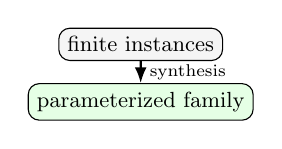
\begin{tikzpicture}[node distance=.32cm, scale=.88, transform shape]
        \node[smallbox, fill=gray!8] (inst) {finite instances};
        \node[smallbox, fill=green!10, below=of inst] (fam) {parameterized family};
        \draw[line] (inst) -- node[right, font=\scriptsize] {synthesis} (fam);
      \end{tikzpicture}
    \column{.61\textwidth}
      {\small
      \[
        k\in K\ \land\
        \forall j.\ 0\le j<k\Rightarrow\varphi_2(j)
        \ \land\ \varphi_3(k)
      \]
      }
      \vspace{-0.55em}
      {\scriptsize The paper synthesizes changing numeric terms, typically using an affine form $a\cdot k+b$.}
  \end{columns}
\end{frame}


\begin{frame}{What becomes smaller?}
  \begin{columns}[T,onlytextwidth]
    \column{.46\textwidth}
      \begin{block}{Standard merge}
        {\scriptsize
        \[
          pc=pc_0\lor pc_1\lor pc_2
        \]
        \[
        \begin{aligned}
          matches={}&ite(pc_0,0,\ ite(pc_1,1,2))\\[0.25em]
          i={}&ite(pc_0,i_0,\\
              &\quad ite(pc_1,i_0+1,i_0+2))
        \end{aligned}
        \]
        }
      \end{block}
    \column{.52\textwidth}
      \begin{block}{Pattern-based merge}
        {\scriptsize
        \[
          k\in\{0,1,2\}\quad(0\le k\le2)
        \]
        \[
          \forall j.\ 0\le j<k \Rightarrow
          (i_0+j<n\land target[j]=i_0+j)
        \]
        \[
          \neg(i_0+k<n)
        \]
        \[
          matches=k,\qquad i=i_0+k
        \]
        }
      \end{block}
  \end{columns}

  \vspace{-0.35em}
  \begin{center}
    \small
    $k$ identifies the selected path case; the same $k$ synthesizes the corresponding store values.\\[0.15em]
    The compact path constraint is equisatisfiable with the standard merge, and store values agree under the corresponding value of k.
  \end{center}

  \vspace{-0.55em}
  {\scriptsize If pattern synthesis fails, use standard merging. If one store value cannot be expressed as $t(k)$, retain its ordinary \texttt{ite}.}
  \sourcefoot{Trabish et al., \emph{State Merging with Quantifiers in Symbolic Execution}.}
\end{frame}


\begin{frame}[fragile]{Back to the project: MIR loop preview}
  \begin{columns}[T,onlytextwidth]
    \column{.42\textwidth}
      \textbf{Scalar MIR skeleton}\\[-0.15em]
\begin{lstlisting}[style=mircode,basicstyle=\ttfamily\fontsize{5.3}{5.8}\selectfont]
matches <-- 0
Lloop:
  ifFalse i < n goto Lend
  ifFalse target == i goto Lskip
  matches <-- +, matches, 1
  goto Lnext
  Lskip: matches <-- +, matches, 0

Lnext:
  i <-- +, i, 1
  goto Lloop

Lend: return matches
\end{lstlisting}
      \vspace{0.1em}
      {\scriptsize The scalar loop is a structural preview, not a full quantified merge.}
    \column{.56\textwidth}
      \textbf{Structural roles recovered by the dump}\\[-0.15em]
      \begin{center}
      \scriptsize
      \begin{tabular}{|l|l|}
        \hline
        MIR evidence & Structural role\\
        \hline
        \texttt{i < n} & loop guard\\
        \hline
        \texttt{target == i} & repeated symbolic branch\\
        \hline
        \texttt{matches + 1} & guarded accumulator\\
        \hline
        \texttt{i + 1} & induction update\\
        \hline
        \texttt{goto Lloop} & back edge\\
        \hline
      \end{tabular}
      \end{center}

      \vspace{-0.25em}
      \textbf{Candidate indexed family}\\[-0.4em]
      {\scriptsize
      \[
      \begin{array}{ll}
      guard(k) & i_0+k<n\\
      branch(k) & target=i_0+k\\
      induction(k) & i=i_0+k\\
      accumulator & matches
      \end{array}
      \]
      }
  \end{columns}

  \vspace{-0.5em}
  \begin{center}
    \scriptsize
    MIR structure $\rightarrow$ candidate repeated family $\rightarrow$ formula and store synthesis $\rightarrow$ quantified merged state
  \end{center}
\end{frame}






\begin{frame}{Beyond scalar MIR: where complexity moves}
  \centering
  \resizebox{.96\linewidth}{!}{%
  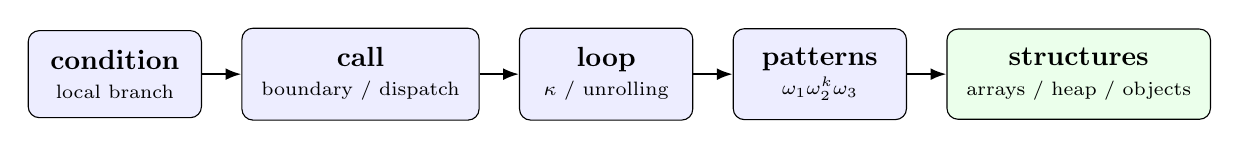
\begin{tikzpicture}[node distance=0.58cm and 0.50cm]
    \node[qbox, fill=blue!7, minimum width=2.20cm] (cond) {\textbf{condition}\\[-0.15em]\scriptsize local branch};
    \node[qbox, fill=blue!7, right=of cond, minimum width=2.20cm] (call) {\textbf{call}\\[-0.15em]\scriptsize boundary / dispatch};
    \node[qbox, fill=blue!7, right=of call, minimum width=2.20cm] (loop) {\textbf{loop}\\[-0.15em]\scriptsize $\kappa$ / unrolling};
    \node[qbox, fill=blue!7, right=of loop, minimum width=2.20cm] (pat) {\textbf{patterns}\\[-0.15em]\scriptsize $\omega_1\omega_2^k\omega_3$};
    \node[qbox, fill=green!8, right=of pat, minimum width=2.45cm] (struct) {\textbf{structures}\\[-0.15em]\scriptsize arrays / heap / objects};
    \draw[line] (cond) -- (call);
    \draw[line] (call) -- (loop);
    \draw[line] (loop) -- (pat);
    \draw[line] (pat) -- (struct);
  \end{tikzpicture}}

  \vspace{0.55em}
  \begin{columns}[T,onlytextwidth]
    \column{.49\textwidth}
      \begin{block}{Harder to model}
        \scriptsize aliasing, bounds, object fields, heap updates
      \end{block}
    \column{.49\textwidth}
      \begin{block}{More structure to exploit}
        \scriptsize sharing, summaries, method regions, array patterns
      \end{block}
  \end{columns}

  \vspace{0.2em}
  \begin{columns}[T,onlytextwidth]
    \column{.49\textwidth}
      \begin{block}{What real engines carry}
        \scriptsize
        \begin{itemize}\itemsep0.15em
          \item KLEE / quantified: arrays, memory objects, solver terms
          \item Veritesting / Java Ranger: regions, calls, dispatch
          \item Efficient merging: store differences, hot variables, query cost
        \end{itemize}
      \end{block}
    \column{.49\textwidth}
      \begin{block}{Limit of this MIR dump}
        \scriptsize
        Mostly scalar variables and CFG dependencies. Memory, aliasing, fields, and heap-shaped updates are only approximated here.
      \end{block}
  \end{columns}

  \vspace{0.1em}
  \centering
  {\scriptsize Next target: represent program structure better, not just shorten formulas.}
\end{frame}

\begin{frame}{Main sources}
  \scriptsize
  \begin{sourcespaperblock}{Papers}
    \begin{enumerate}
      \item C. Cadar, D. Dunbar, and D. Engler. \emph{KLEE: Unassisted and Automatic Generation of High-Coverage Tests for Complex Systems Programs}. OSDI, 2008.
      \item V. Kuznetsov, J. Kinder, S. Bucur, and G. Candea. \emph{Efficient State Merging in Symbolic Execution}. PLDI, 2012.
      \item T. Avgerinos, A. Rebert, S. K. Cha, and D. Brumley. \emph{Enhancing Symbolic Execution with Veritesting}. ICSE, 2014.
      \item V. Sharma, S. Hussein, M. W. Whalen, S. McCamant, and W. Visser. \emph{Java Ranger: Statically Summarizing Regions for Efficient Symbolic Execution of Java}. ESEC/FSE, 2020.
      \item D. Trabish, N. Rinetzky, S. Shoham, and V. Sharma. \emph{State Merging with Quantifiers in Symbolic Execution}. 2023.
    \end{enumerate}
  \end{sourcespaperblock}
  \vspace{0.25em}
  \begin{sourcesprojectblock}{Project artifacts}
    \href{https://github.com/yaryabtsev/compilers-course}{\texttt{github.com/yaryabtsev/compilers-course}}\\[0.25em]
    MIR dumps, CFGs, QCE tables, and merge-risk reports.
  \end{sourcesprojectblock}
\end{frame}

\end{document}
